\documentclass[border=8pt]{standalone}
\usepackage{amsmath,amssymb}
\usepackage{tikz}
\usetikzlibrary{arrows.meta,calc,decorations.pathreplacing,patterns,shapes.geometric,positioning,shadings,plotmarks}

\begin{document}
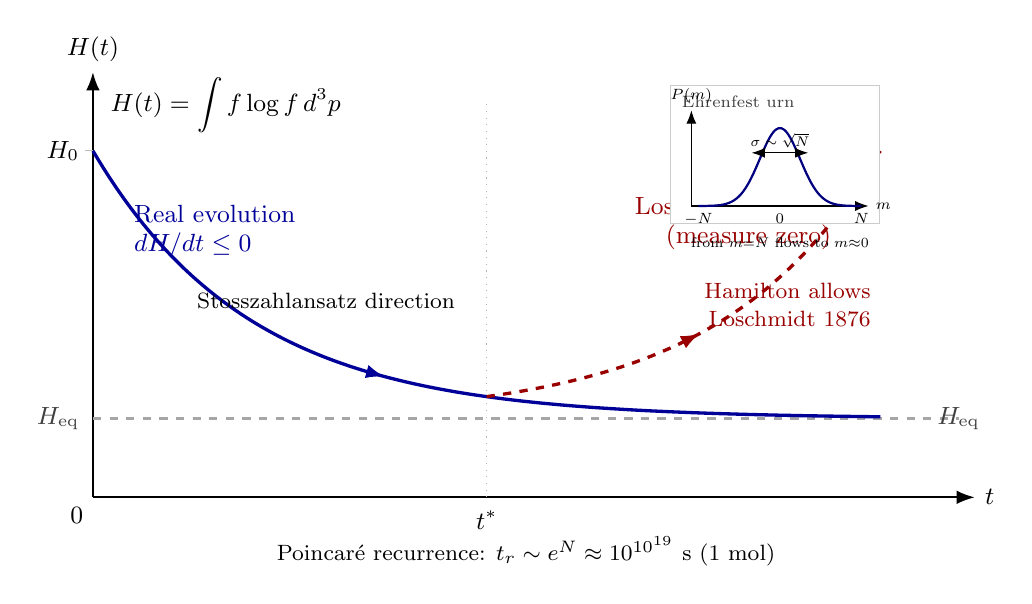
\begin{tikzpicture}[>=Latex, font=\small]

% ============== MAIN PANEL: H(t) curve ==================
% Coordinates: x-axis from 0 to 10, y-axis from 0 to 5
% t* at x=5 (mirror axis)
% H_eq at y=1, H_0 at y=4.4

% Background grid (subtle)
\draw[white] (0,0) rectangle (11.5,5.6);

% Axes
\draw[->, thick] (0,0) -- (11.2,0) node[right] {$t$};
\draw[->, thick] (0,0) -- (0,5.4) node[above] {$H(t)$};

% Axis ticks
\draw (0,0) node[below left] {$0$};

% Equilibrium dashed line
\draw[dashed, gray!70, thick] (0,1) -- (11,1);
\node[anchor=west, gray!50!black] at (10.6,1) {\small $H_{\text{eq}}$};
\node[anchor=east, gray!50!black] at (-0.05,1) {\small \(H_{\text{eq}}\)};

% H_0 marker on left axis
\node[anchor=east] at (-0.05,4.4) {\small $H_0$};
\draw[gray!50] (-0.1,4.4) -- (0,4.4);

% Mark t*
\draw[dotted, gray!60] (5,0) -- (5,5);
\node[below] at (5,-0.05) {\small $t^{*}$};

% Real evolution: monotone exponentially decreasing curve from (0,4.4) to (10, 1.05)
% H(t) = H_eq + (H_0 - H_eq) * exp(-t/tau), tau = 2
% At t=0: 4.4; t=5: 1 + 3.4*exp(-2.5) = 1.279; t=10: 1+3.4*exp(-5)=1.023
\draw[very thick, blue!60!black, smooth, samples=80, domain=0:10]
  plot (\x, {1 + 3.4*exp(-\x/2)});

% Loschmidt mirror: rises from t* point upward, mirrored about t*
% At time t* the real curve hits H(t*) = 1 + 3.4*exp(-2.5) ~= 1.279
% Mirror: for t in [t*, t*+5], H_mirror(t) = real(2*t* - t) reversed?
% Actually we want a curve symmetric about t* that goes back up. Starting at (t*, H(t*)) and going up to match (10, ~4.4)
% Use H_m(t) = 1 + 3.4*exp(-(2*t* - t)/2) for t > t*
% At t=5: 1 + 3.4*exp(-2.5) = 1.279
% At t=10: 1 + 3.4*exp(0) = 4.4
\draw[very thick, red!60!black, dashed, smooth, samples=80, domain=5:10]
  plot (\x, {1 + 3.4*exp(-(10-\x)/2)});

% Also extend the mirror going backward in time? No - mirror lives only after t*
% Add mirror also from start: full Loschmidt symmetric mirror going from t=0 at H=1.05 upward to t* then back down
% (the symmetric reflection of the real curve about the horizontal axis t=t*).
% That visual may be too busy; keep just the rising mirror after t*.

% Labels for curves
\node[blue!60!black, anchor=west] at (0.4,3.6) {\small Real evolution};
\node[blue!60!black, anchor=west] at (0.4,3.2) {\small \(dH/dt \le 0\)};

\node[red!60!black, anchor=east] at (9.5,3.7) {\small Loschmidt mirror};
\node[red!60!black, anchor=east] at (9.5,3.3) {\small (measure zero)};

% Arrow on real curve showing direction
\draw[->, thick, blue!60!black] (3.5,1+3.4*0.1738) -- (3.7,{1+3.4*exp(-3.7/2)});

% Arrow on mirror curve showing direction
\draw[->, thick, red!60!black, dashed] (7.5,{1+3.4*exp(-2.5/2)}) -- (7.7,{1+3.4*exp(-2.3/2)});

% Stosszahlansatz arrow
\node[align=center, anchor=west] at (1.2,2.5) {\footnotesize Stosszahlansatz direction};

% Hamilton-allowed note for mirror
\node[align=center, anchor=south east, red!60!black] at (10.0,2.4) {\footnotesize Hamilton allows};
\node[align=center, anchor=south east, red!60!black] at (10.0,2.05) {\footnotesize Loschmidt 1876};

% Definition of H
\node[anchor=north west] at (0.1,5.45) {\small $H(t)=\displaystyle\int f\log f\,d^{3}p$};

% Bottom note: Poincare recurrence
\node[anchor=south, align=center] at (5.5,-1.0)
  {\footnotesize Poincar\'e recurrence: $t_{r}\sim e^{N}\approx 10^{10^{19}}$ s (1 mol)};

% ============== INSET: Ehrenfest urn ==================
% Place at top-right
\begin{scope}[shift={(7.6,3.7)}, scale=0.45, every node/.style={scale=0.85}]
  % Inset frame
  \draw[gray!40, thin, fill=white] (-0.6,-0.5) rectangle (5.3,3.4);
  \node[anchor=north west, gray!50!black] at (-0.5,3.35) {\scriptsize Ehrenfest urn};

  % axes
  \draw[->] (0,0) -- (5.0,0) node[right, scale=0.9] {\scriptsize $m$};
  \draw[->] (0,0) -- (0,2.7) node[above, scale=0.9] {\scriptsize $P(m)$};

  % center mark
  \node[below, scale=0.9] at (2.5,0) {\scriptsize $0$};
  \node[below, scale=0.9] at (0.2,0) {\scriptsize $-N$};
  \node[below, scale=0.9] at (4.8,0) {\scriptsize $N$};

  % Bell curve: P(m) = 2.2 * exp(-((m-2.5)/0.8)^2)
  \draw[thick, blue!50!black, smooth, samples=60, domain=0.2:4.8]
    plot (\x, {2.2*exp(-((\x-2.5)/0.8)^2)});

  % sigma indicator
  \draw[<->, thin] (1.7,1.5) -- (3.3,1.5);
  \node[scale=0.85] at (2.5,1.85) {\scriptsize $\sigma\sim\sqrt{N}$};

  % note
  \node[align=center, scale=0.85, anchor=north] at (2.5,-0.7)
    {\scriptsize from $m{=}N$ flows to $m{\approx}0$};
\end{scope}

\end{tikzpicture}
\end{document}
